
\section{Introduction}
\label{sec:intro}

\begin{figure}[t]
  \begin{center}
    
\includegraphics[width=0.95\columnwidth]{figs/workflow.eps}
    \caption{Workflow}
    \label{fig:Normal workflow for most multi-tier service oriented systems}
  \end{center}
\end{figure}

\begin{figure*}[t]
  \begin{center}
    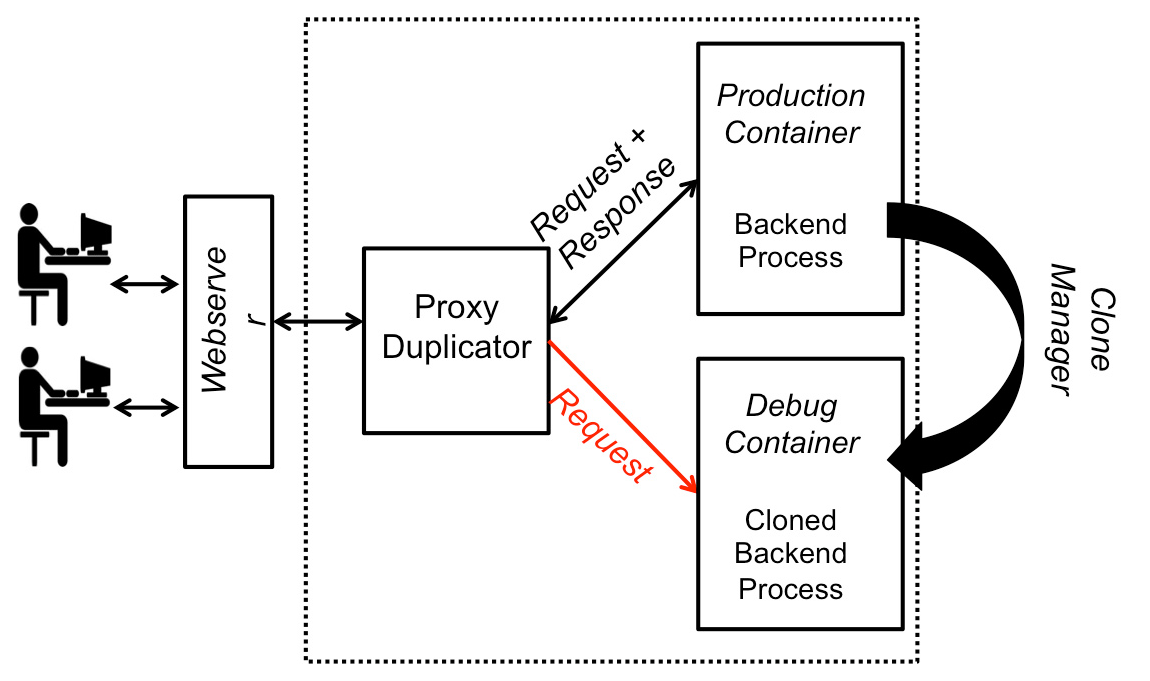
\includegraphics[width=0.8\textwidth]{figs/workflow2.eps}
    \caption{Workflow}
    \label{fig:Backend wrapped around with Parakishan Run-time}
  \end{center}
\end{figure*}

As application software grows and gets more complicated, testing large scale applications has become increasingly important. 
However, it is often impossible to recreate realistic workloads in an offline development environment for large scale multi-tier or cloud based applications.
On the other hand, there has been an equally impressive increase in the scale of computing resources, and distributed scalability of infrastructure.
This often allows for redundant computation, which can be used for testing purposes. 
Leveraging this abundance of resource we present a testing harness which allows the user to dynamically insert test cases in a production environment.

Our tool called \texttt{Parikshan}\footnote{Parikshan is the sanskrit word for testing} which allows capturing the context of application, and allows for a test-case to be run without effecting the sanctity of the actual application. 
This is achieved by using dynamic instrumentation mechanisms to initiate a VM from forking off an executed state and encapsulating the forked execution in a VM.
The user can pre-define probe points for dynamically inserting test-cases (by default the entry and exit of each function) is considered a probe point.
Since the test is executed in a VM it acts like a sandbox which restricts it from causing any perturbation to the state of the parent process


The key contributions of this paper are:

\begin{itemize}
\item Our tool provides a sandbox environment to execute test cases in the production environment. 
This allows for a safe and secure test harness which does not effect the production state, and allows the application to safetly proceed in it's execution.
\item We allow for dynamic insertion of the test case, and safetly capturing the context of the application. 
\texttt{Zero-Probe Effect} probe points are added to the application which can be activated to insert test cases using ptrace\cite{ptrace}.
The use of dynamic instrumentation capability to add test cases in an application is an extension of our previous work of a dynamic instrumentation tool iProbe \cite{iProbe}
\end{itemize}

The authors previous work in in-vivo testing\cite{invite} explored testing in the wild by initiating test cases in the production environment and sharing the load across several instances of deployed application.
This approach adds test-cases in predetermined functions before starting the execution of the process, and periodically executes them in the run-time environment based on a probabilistic function. 

\cite{dapper}

\subsection{Impact}
\label{sec:impact}

The impact of sandbox testing can be seen in several different ways

\begin{itemize}
  \item \textbf{Sandbox Live Testing}
    One of the key motivations leading to \emph{Parikshan} is to provide a harness to allow the user to test real, live implementations. 


  \item \textbf{Fault Tolerance}
  \item \textbf{Verification}
  \item \textbf{Integration Testing}
\end{itemize}

